% This is samplepaper.tex, a sample chapter demonstrating the
% LLNCS macro package for Springer Computer Science proceedings;
% Version 2.20 of 2017/10/04
%
\documentclass[runningheads]{llncs}
%
\usepackage{graphicx}
\usepackage{listings}
\usepackage{xcolor}

\definecolor{codegreen}{rgb}{0,0.6,0}
\definecolor{codegray}{rgb}{0.5,0.5,0.5}
\definecolor{codepurple}{rgb}{0.58,0,0.82}
\definecolor{backcolour}{rgb}{0.95,0.95,0.92}

\lstdefinestyle{mystyle}{
    backgroundcolor=\color{backcolour},
    commentstyle=\color{codegreen},
    keywordstyle=\color{magenta},
    numberstyle=\tiny\color{codegray},
    stringstyle=\color{codepurple},
    basicstyle=\ttfamily\footnotesize,
    breakatwhitespace=false,
    breaklines=true,
    captionpos=b,
    keepspaces=true,
    numbers=left,
    numbersep=5pt,
    showspaces=false,
    showstringspaces=false,
    showtabs=false,
    tabsize=2
}
\lstset{style=mystyle}

\begin{document}
%
\title{Augraphy: Data Augmentation for \\Document Images\thanks{Supported by Sparkfish LLC.}}
\author{Alexander Groleau\inst{1} \and
Kok Wei Chee \and
Stefan Larson\inst{2}}
%
\authorrunning{A. Groleau et al.}
% First names are abbreviated in the running head.
% If there are more than two authors, 'et al.' is used.
%
\institute{Sparkfish, Addison TX, USA\\\and
  SkySync, Ann Arbor MI, USA\\
  \and
  \email{ck91wei@gmail.com}}
\maketitle
%
\begin{abstract}
This short paper introduces \emph{Augraphy}, a Python package for data augmentation pipelines for document image analysis.
Augraphy uses many different augmentation strategies to produce augmented versions of clean document images that appear as if they have been distorted due to noisy paper printing, faxing, scanning, or copy machine processes.

\keywords{Document Analysis \and Denoising \and Data Augmentation.}
\end{abstract}
%
%
%
\section{Introduction}
Data augmentation is a widely used strategy in various areas of machine learning, including computer vision, image processing, natural language processing, and audio applications. Data augmentation can be used to generate new training samples data by applying transformations, rotations, noise, and other modifications to training data.
Alternatively, data augmentation can be used to create noisy or challenging evaluation data from clean data, in which case it can be used for robustness testing or image denoising.\\

This paper introduces Augraphy,\footnote{https://github.com/sparkfish/augraphy} a Python library for document image data augmentation.
Augraphy uses highly-configurable pipelines to apply adjustments to document images to create augmented versions that appear old or noisy, as if they had been printed on dirty laser or inkjet printers, scanned by dirty or low-quality office scanners, or otherwise mistreated by real-world paper handling office equipment.
This paper highlights some of the features of Augraphy, and demonstrates how it can be used effectively to produce challenging synthetic document denoising data.
\begin{figure}
    \centering
    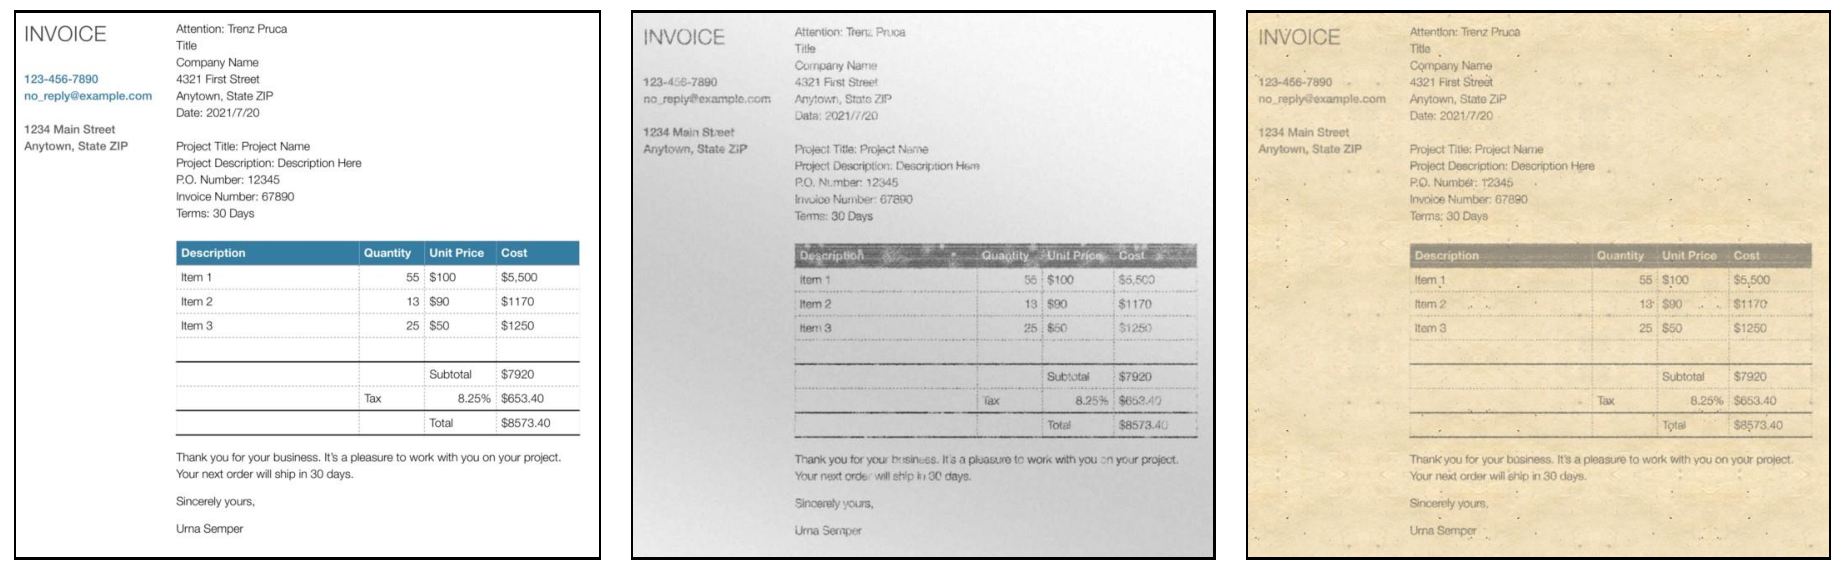
\includegraphics[width=\linewidth]{augraphy_3panel.pdf}
    \caption{Example input image (left) with two augmented versions (middle and right).}
    \label{fig:3panel}
\end{figure}

\section{Augraphy}
%\subsection{Related Work}
\paragraph{\textbf{Related Work.~~}}
 Several data augmentation libraries exist for image tasks. General purpose image augmentation libraries include Albumentations
 %\footnote{\texttt{\href{https://albumentations.ai/}{albumentations.ai}}}
 \cite{albumentations}, Augmentor
 %\footnote{\texttt{\href{https://augmentor.readthedocs.io/en/master/}{augmentor.readthedocs.io}}}
 \cite{augmentor}, Augly
 %\footnote{\texttt{\href{https://github.com/facebookresearch/AugLy}{github.com/facebookresearch/AugLy}}}
 \cite{augly}, and imgaug
 %\footnote{\texttt{\href{https://imgaug.readthedocs.io/en/latest/}{imgaug.readthedocs.io}}}
 \cite{imgaug}.
Augmentation techniques from these general purpose libraries include rotations, translations, warps, and color transformations, yet none of these libraries provide augmentations targeted at imitating the types of transformations seen in document analysis corpora.


A notable exception is DocCreator
%\footnote{\texttt{\href{https://doc-creator.labri.fr/}{doc-creator.labri.fr}}}
\cite{doccreator}, which is a document synthesizing tool that provides several transformation strategies as part of its synthesis pipeline.
DocCreator's augmentations target imitating artefacts seen in historical (e.g., ancient or medieval) manuscripts, and hence do not address more modern causes of noise, such as noise introduced by document scanners.
DocCreator is written in C++ and is meant to be used as a what-you-see-is-what-you-get tool; with no scripting or API interface, it is not easily amenable to being used in broader machine learning model development pipelines.
In contrast, Augraphy is written in Python and has a simple interface to allow for seamless use with other Python libraries and data pipelines.

%\subsection{The Augraphy Package}
\paragraph{\textbf{The Augraphy Package.~~}}
Augraphy is a lightweight Python package. It is registered on the Python Package Index (PyPI) and can be installed using
\texttt{pip install augraphy}~.
%$$
%\texttt{pip install augraphy}
%$$
Augraphy requires only a few other commonly-used Python scientific computing or image handling packages in order to run, such as NumPy and Pillow.
Augraphy has been tested on Windows, Linux, and Mac computing environments.
Listing 1 shows how easy it is to get Augraphy up and running to create a straightforward augmentation pipeline and apply it to an image.

\begin{lstlisting}[language=Python, caption=Transforming an image with Augraphy.]
import augraphy; import cv2
pipeline = augraphy.default_augraphy_pipeline()
img = cv2.imread("image.png")
data = pipeline.augment(img)
augmented = data["output"]
\end{lstlisting}\label{sample-code}
% reference to this listing seems broken, and why is it printing 1.1 and not just 1?

Examples of output generated by Augraphy can be seen in Figure~\ref{fig:3panel}, which shows augmentations mimicking low printer ink and fuzzy, low-resolution text (middle image), and other paper surfaces (right image).
We also show several of Augraphy's individual augmentation features in Figure~\ref{fig:augmentations}.
Importantly, these individual augmentation strategies can be composed together in an augmentation pipeline to create even more realistic looking, noisy output.

\begin{figure}
    \centering
    %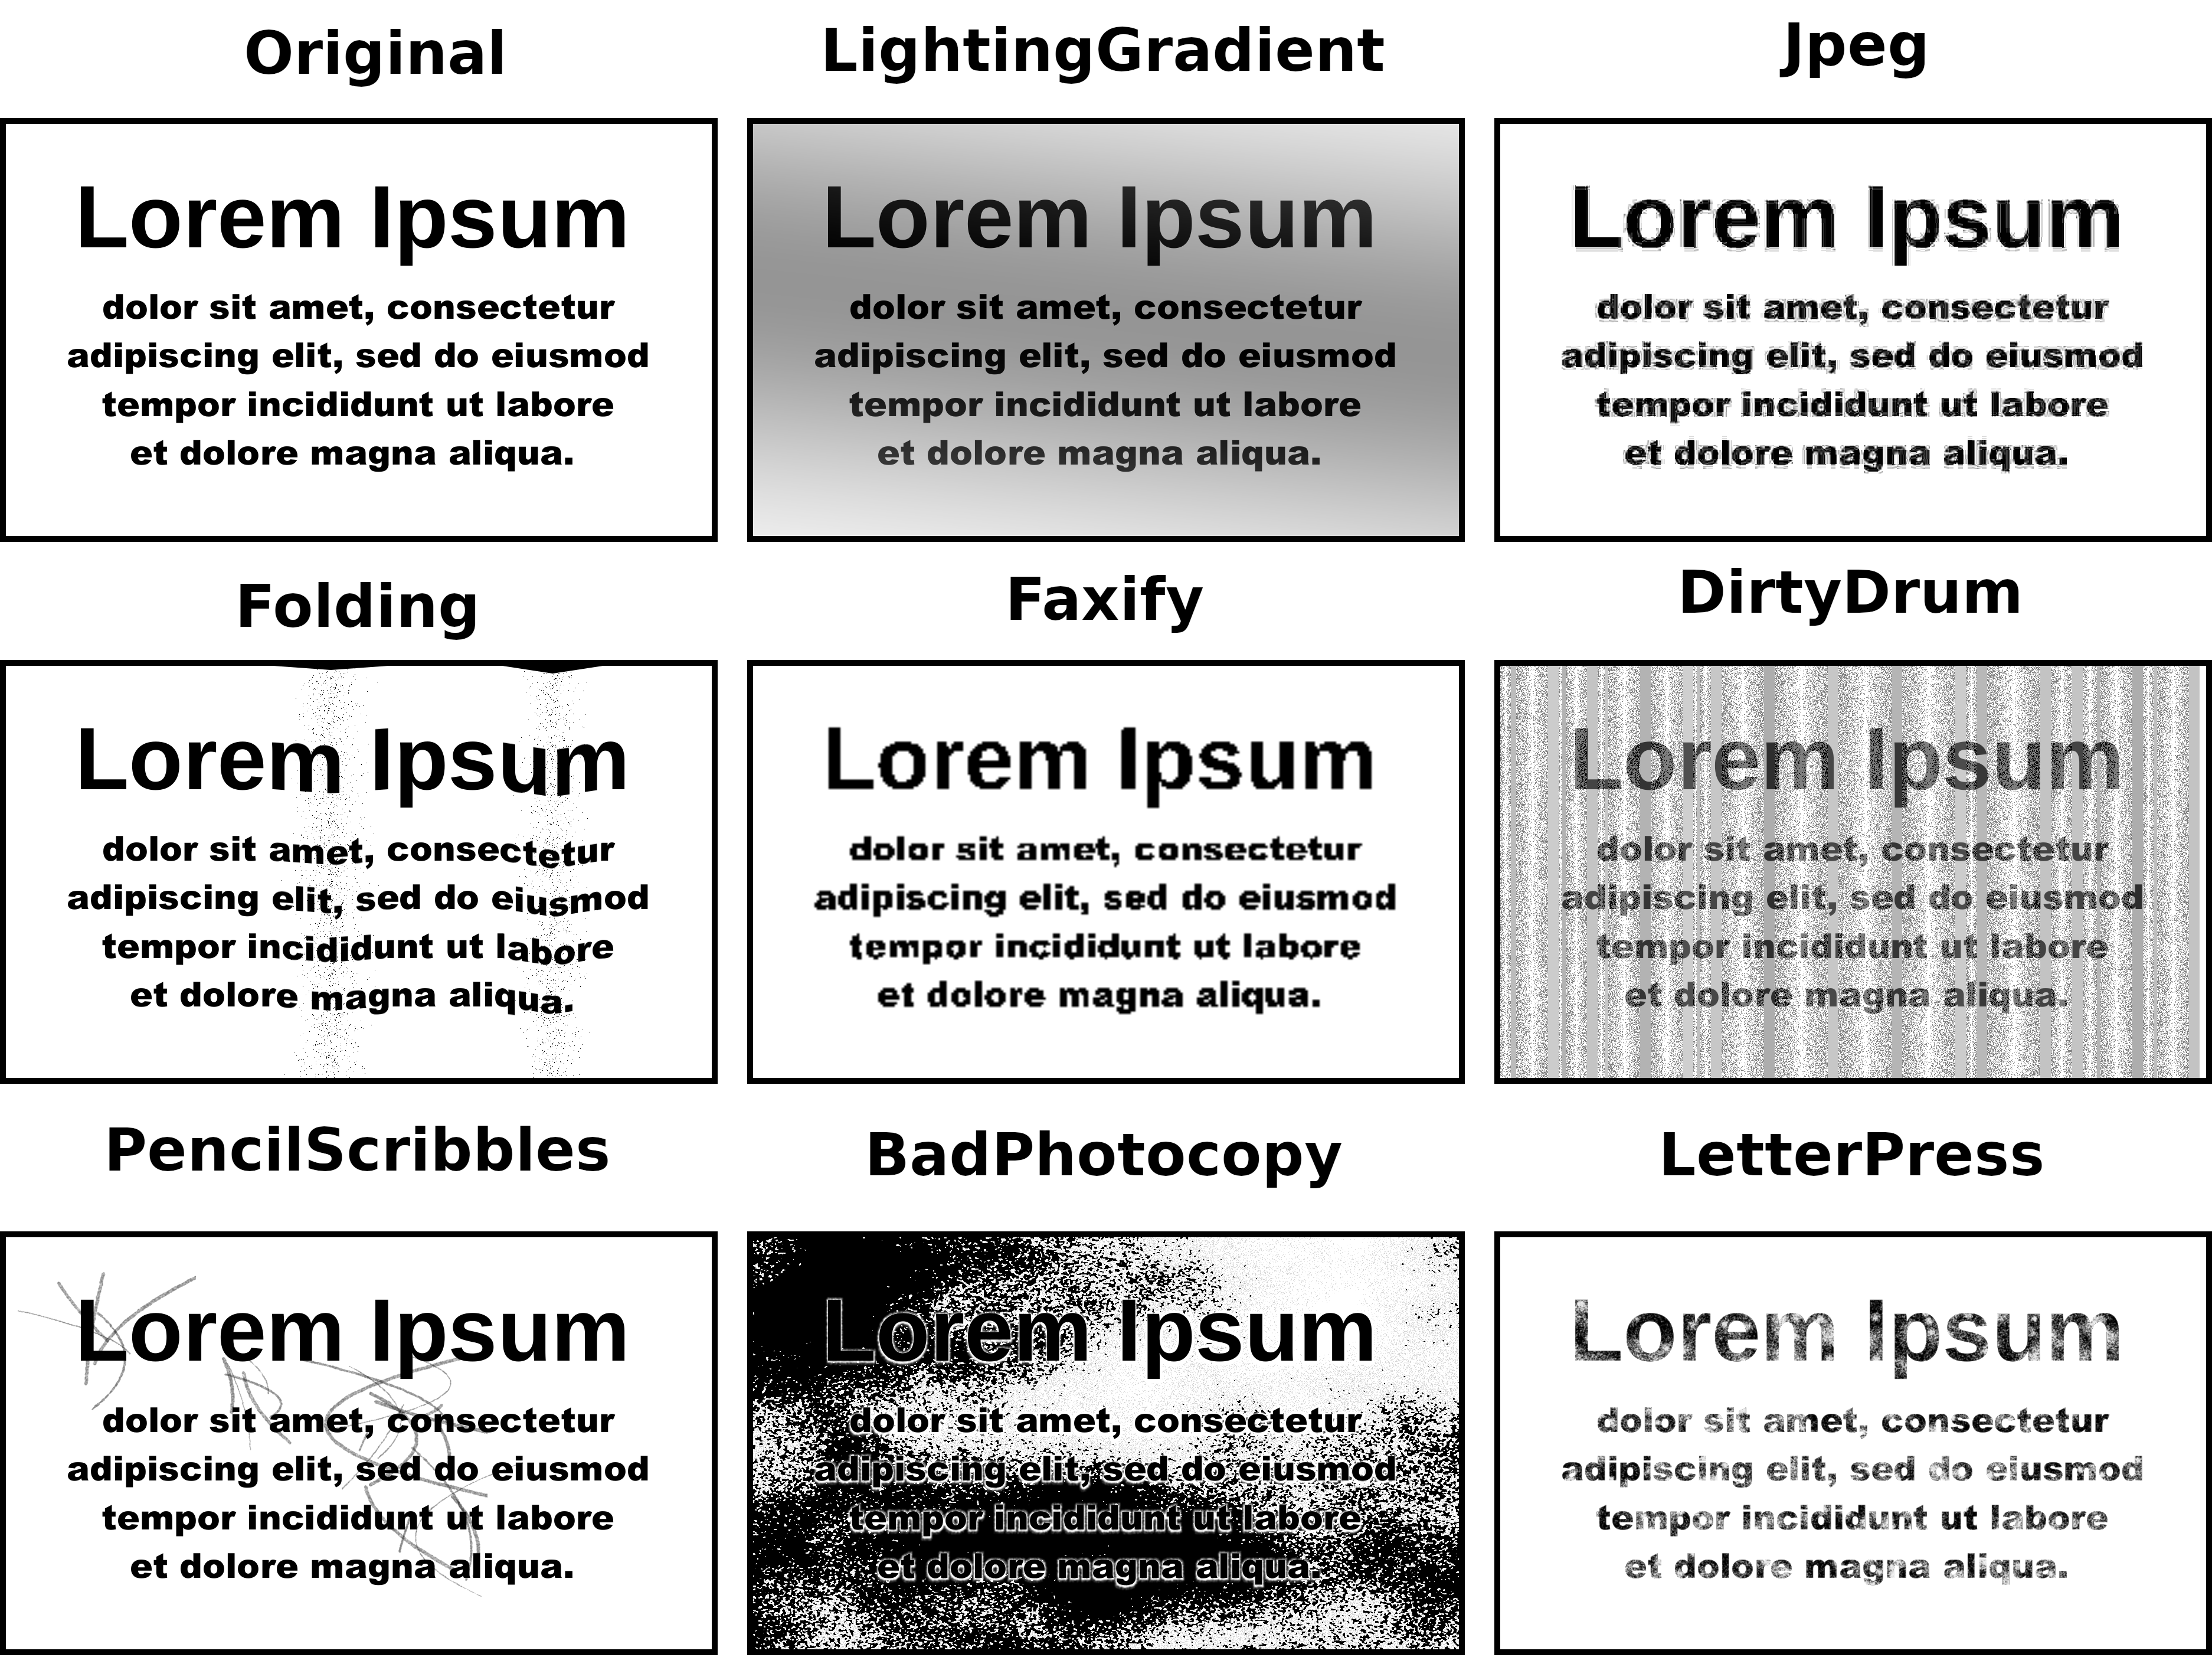
\includegraphics[width=0.75\textwidth]{augraphy_augmentations.png}
    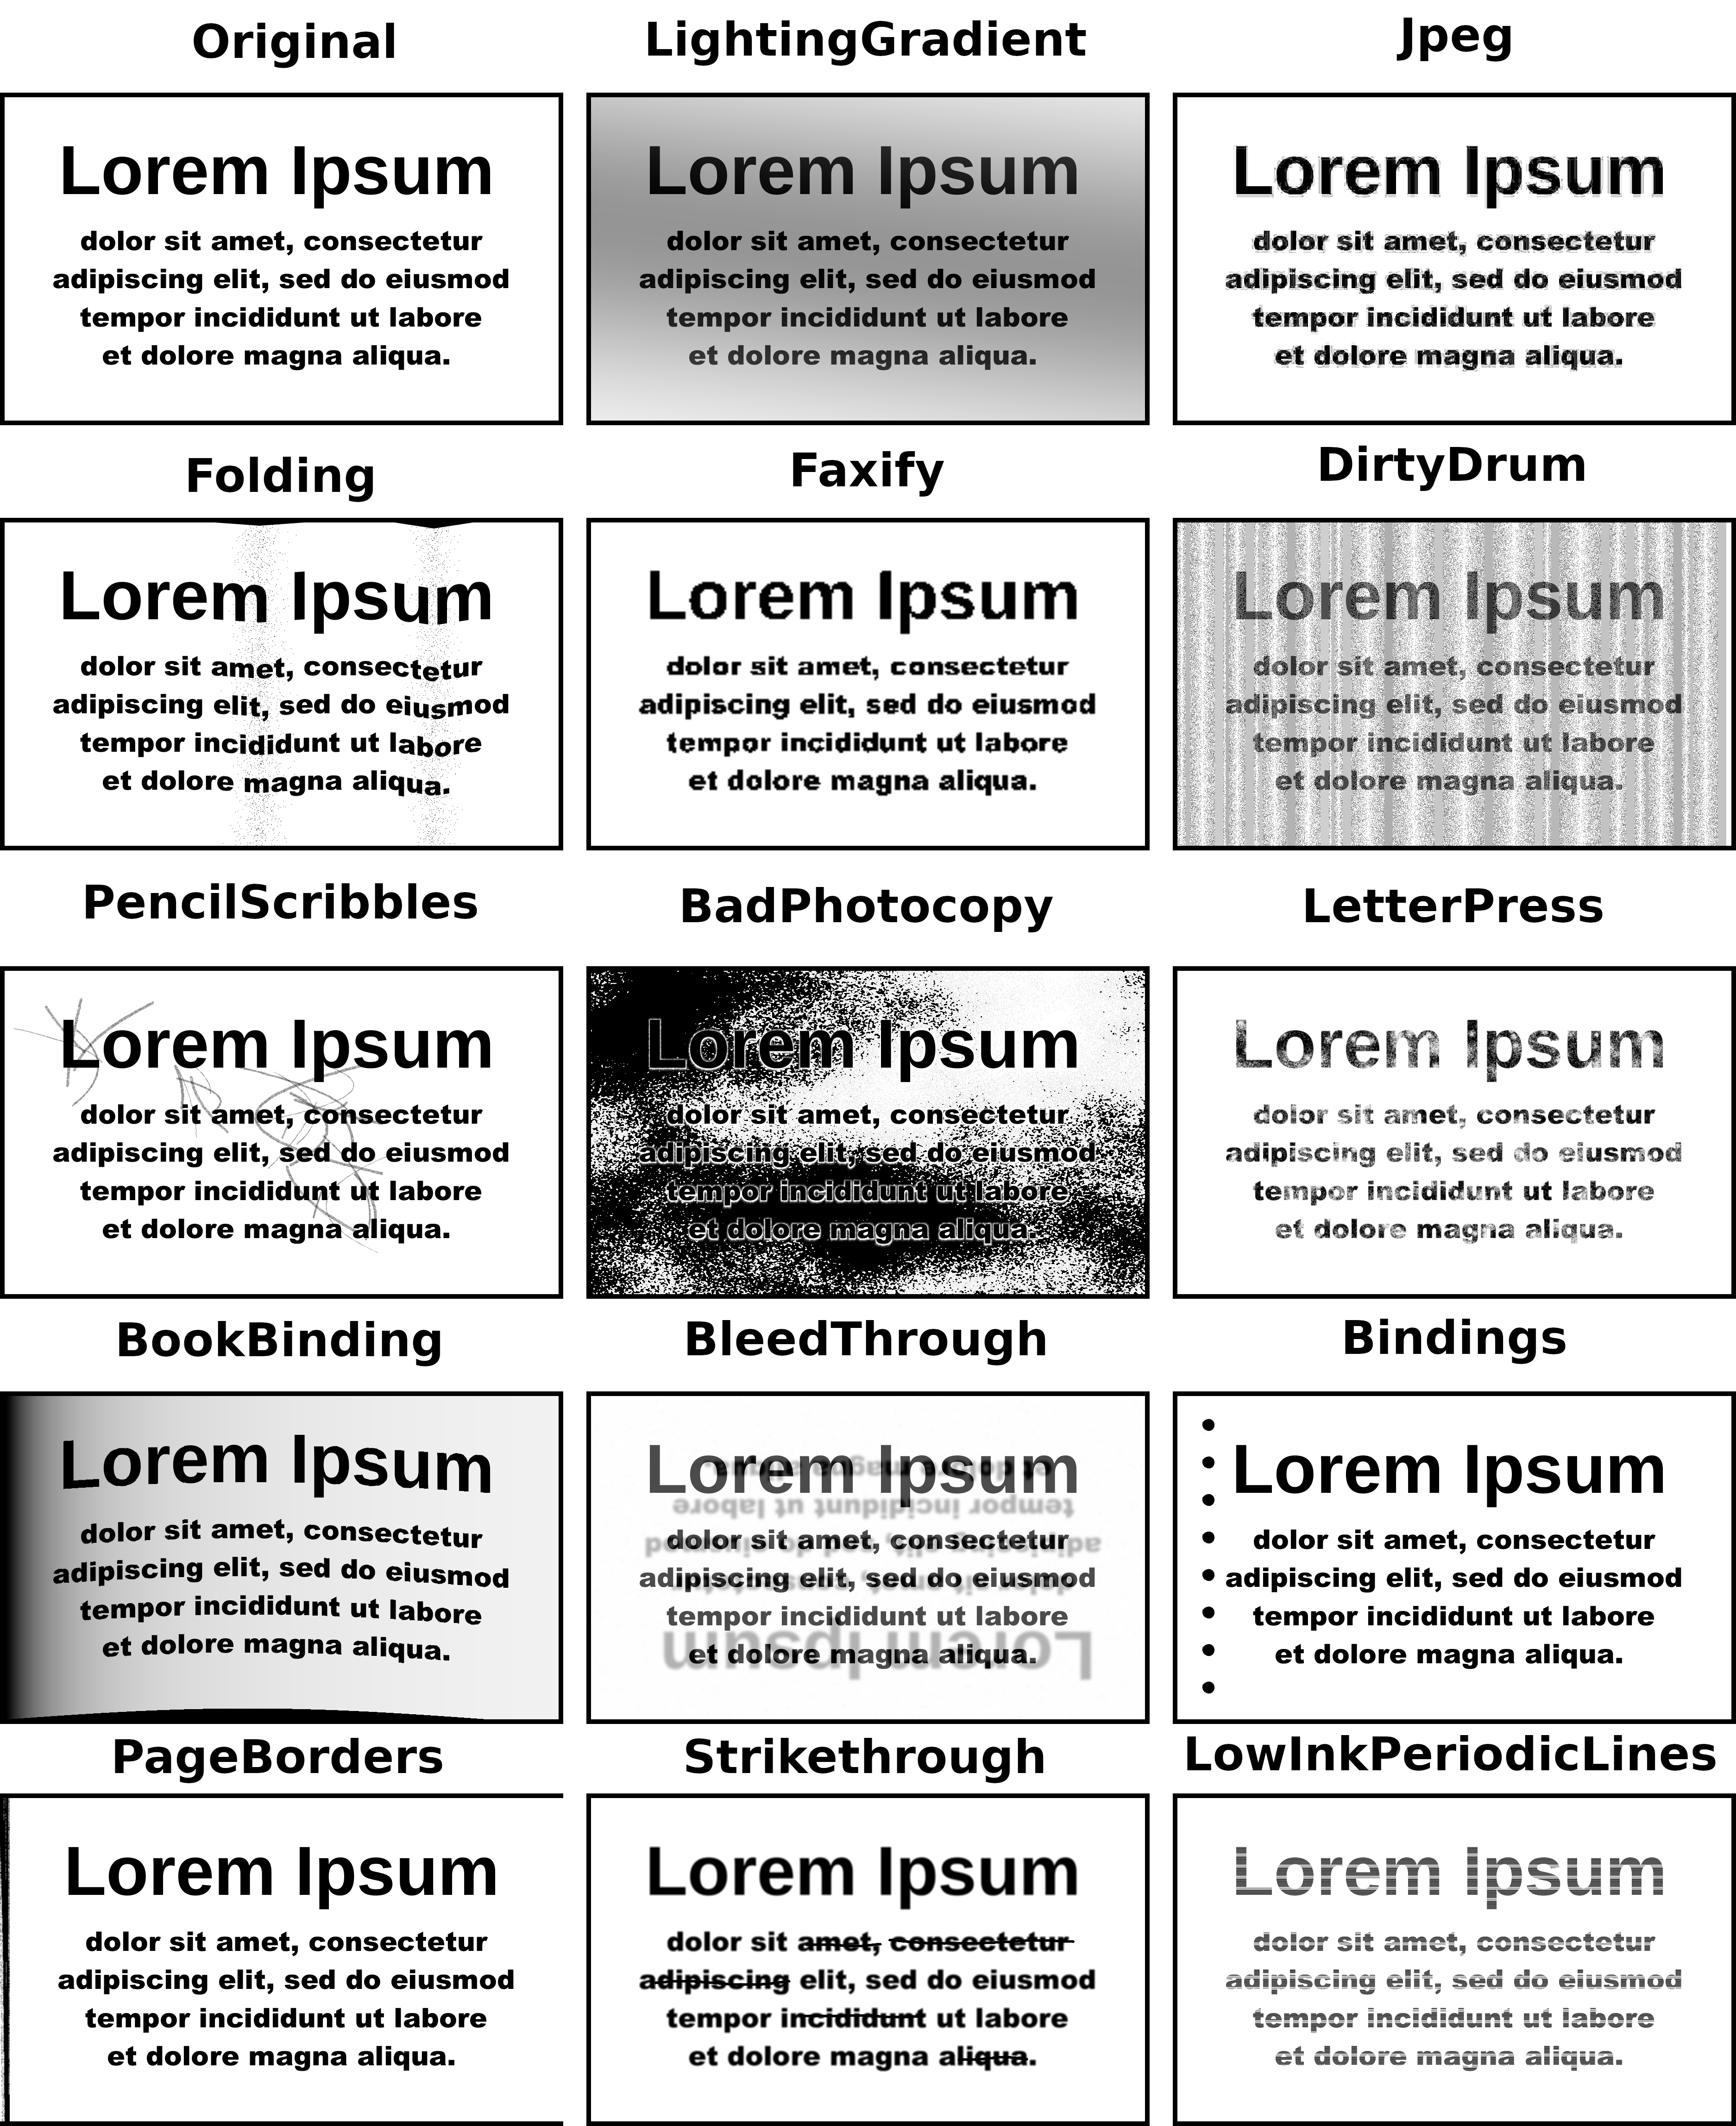
\includegraphics[width=0.72\textwidth]{augraphy_various.png}
    \caption{Various individual augmentation types available in Augraphy. These individual augmentations can also be composed together.}
    \label{fig:augmentations}
\end{figure}




%\subsection{Qualitative Case Study: Document Denoising}
\paragraph{\textbf{Qualitative Case Study: Document Denoising.~~}}
In this section we highlight the effectiveness of Augraphy by creating a new evaluation set for the task of document denoising.
Document denoising is the task of removing noisy artifacts from a document image, and one recent dataset that has emerged for this task is the NoisyOffice dataset \cite{noisyoffice}, which itself generated noisy versions of clean documents by applying several augmentations.
However, both the original documents and the augmentations in NoisyOffice are quite limited, so it is natural to wonder if a model trained on NoisyOffice data can generalize to more diverse data inputs for the denoising task.

\begin{figure}
    \centering
    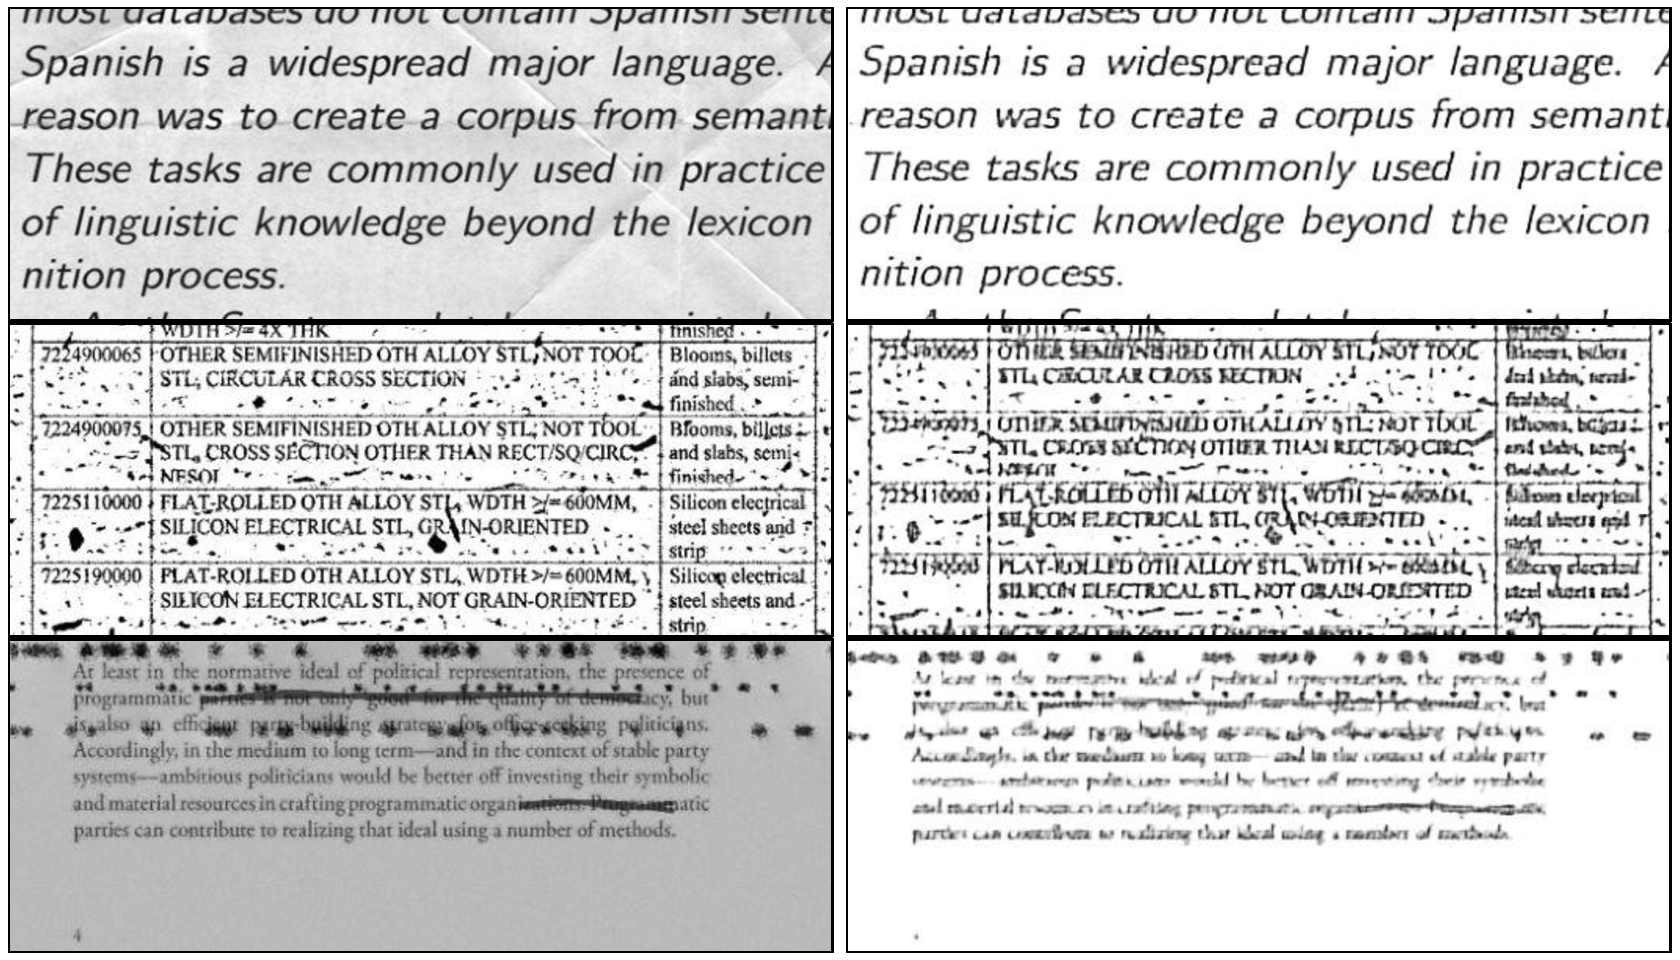
\includegraphics[width=0.9\textwidth]{augraphy_noisy_office_qualitative_comparison_figure.pdf}
    \caption{Inputs (left) and outputs (right) to a denoising model. A NoisyOffice \cite{noisyoffice} sample is shown in the top row. Augraphy samples are shown in the bottom two rows.}
    \label{fig:noisy_office_comparison}
\end{figure}

In Figure~\ref{fig:noisy_office_comparison} we show example test inputs (left) to a convolutional autoencoder, which we trained on the NoisyOffice dataset.
The model's outputs are shown on the right side of Figure~\ref{fig:noisy_office_comparison}.
We see that the model does well on the NoisyOffice input (top row), but underperforms on data that was augmented by Augraphy (bottom two rows), showing that Augraphy's augmentations are effective at producing challenging testing data for analyzing the robustness of denoising models.



\section{Conclusion}
This paper introduces Augraphy, a new data augmentation package for document analysis tasks.

%
% ---- Bibliography ----
%
% BibTeX users should specify bibliography style 'splncs04'.
% References will then be sorted and formatted in the correct style.
%
% \bibliographystyle{splncs04}
% \bibliography{mybibliography}
%
\begin{thebibliography}{8}
\bibitem{augmentor}
Bloice, M., Roth, P., Holzinger, A. Biomedical image augmentation using Augmentor. \emph{Bioinformatics}, 35(21):4522-4524, 2019.

\bibitem{augly}
Papakipos, Z., Bitton, J. AugLy: Data Augmentations for Robustness. \emph{arXiv preprint}, 2022.

\bibitem{albumentations}
Buslaev, A., Iglovikov, V., Khvedchenya, E., Parinov, A., Druzhinin, M., Kalinin, A. Albumentations: Fast and flexible image augmentations. \emph{Information}, 11(2), 2020.

\bibitem{doccreator}
Journet, N., Visani, M., Mansencal, B., Van-Cuong, K., Billy, A. Doccreator: A new software for creating synthetic ground-truthed document images. \emph{Journal of Imaging}, 3(4):62, 2017.

\bibitem{imgaug}
Jung, A., et al. Imgaug. 2020.

\bibitem{noisyoffice}
Castro-Bleda, M., Espa\~{n}a-Boquera, S., Pastor-Pellicer, J., Zamora-Mart\'{i}nez, F. The NoisyOffice Database: a corpus to train supervised machine learning filters for image processing. \emph{The Computer Journal}, 63(11):1658-1667, 2020.






\end{thebibliography}
\end{document}
